\section*{Generating multinormal and multi-student r.v.'s}

\subsection*{Q1}

First we run the following script:

\begin{verbatim}
> set.seed(1)
> sum(duplicated(runif(1e6))) ## = 120
[1] 120
> sum(duplicated(rnorm(1e8))) ## = 0
[1] 0
\end{verbatim}

The function \verb|duplicated| returns a logical array where unique numbers are marked with 0 and duplicates are marked with 1 (the first occurence of the number is marked with a 0). Summming this array thus gives the total number of duplicates. The uniform distribution gives 120 duplicates in a much smaller sample size than the normal distribution, which gives 0 duplicates.

In the assignment, the expected number of different numbers is derived to be 
\begin{equation}
  \E[N_n] = \frac{1 - f^n}{1-f}
\end{equation}

The number of duplicates is then given by 
$n - \E[N_n]$
We run the following script:

\begin{verbatim}
> m <- 2^32;n <- 1e6
> f <- 1 - 1/m
> num_dup_unif <- n - (1-f^n)/(1-f)
> num_dup_unif
[1] 116.3988
\end{verbatim}

The expected result of 116.4 is quite close to the generated result. The outcome of 120 is therefore consistent with the assumption that \verb|runif| produces different values uniformly.

The resolution of \verb|rnorm| is somewhere in the $2^{50}$'s. Directly calculating $1 - f^n$ will give $1$, because f is so close to $1$.
First, we use to approximation given in the assignment.
\begin{equation}
f^n = \left( 1 - \frac{1}{m}\right)^n \approx 1 - \frac{n}{m} + \frac{n^2}{2m^2}
\end{equation}

Inserting this into our equation for the number of different numbers gives
\begin{equation}
\frac{1 - f^n}{1-f} \approx \frac{1 - 1 + \frac{n}{m} - \frac{n^2}{2m^2}}{1- \left(1 - \frac{1}{m}\right)}  = \frac{\frac{n}{m} - \frac{n^2}{2m^2}}{\frac{1}{m}} = n - \frac{n^2}{2m}
\end{equation}

This results in the following equation for the expected number of duplicates.
\begin{equation}
n - \left(n - \frac{n^2}{2m}\right) = \frac{n^2}{2m}
\end{equation}

Next we check in \verb|R| if the number of duplicates is consistent with values for $m$ of $10^{15}$, $10^{16}$, $10^{17}$ or $10^{18}$, when $n$ is $10^8$
\begin{verbatim}
> n_norm <- 1e8
> m_norm <- c(1e15,1e16,1e17,1e18)
> num_dup_norm <- n_norm^2/(2*m_norm)
> num_dup_norm
[1] 5.000 0.500 0.050 0.005
\end{verbatim}

The obtained result seems to be consistent with a resolution of $10^{16}$ or higher.
 
\subsection*{Q2}
The following code is executed in \verb|R|.
\begin{verbatim}
> n <- 200; p <- 0.52
> x <- c(0,cumsum(2*rbinom(n,1,p)-1))
> plot(x, type="l", lwd=1, ylab="state", xlab="step", main="1-dimensional random walk")
\end{verbatim}
This gives the following biased random walk:

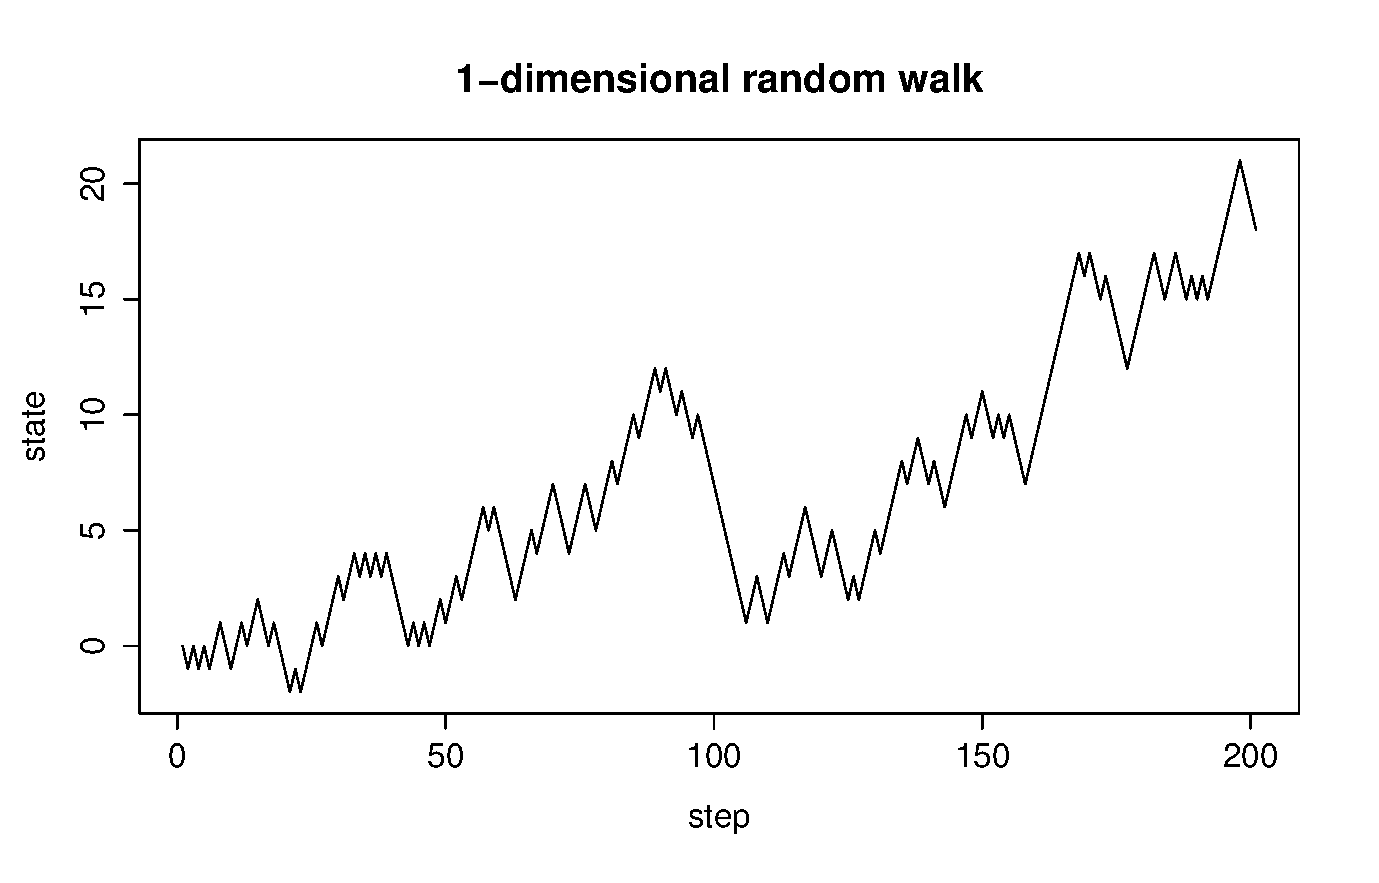
\includegraphics[scale=.6]{NL1_Q2_1D-randomwalk.eps} 

\subsection*{Q3}

Given that $X$, $Y \sim N(0,1)$, we want to transform $(X, Y)$ into $(X, Y^*)$, with $Y^* = aX + bY$, with $a, b$ chosen in such a way that $\Var[Y^*] = 1$ and $r(X, Y^*) = 0.8$.

\begin{align}
r(X, Y^*) & = \frac{\E[X Y^*] - \E[X] \E[Y*]}{\sqrt{\Var[X] \Var[Y^*]}} = \frac{\E[a X^2 + b X Y] - 0 \cdot \E[Y^*]}{\sqrt{1 * 1}} \\
          & = a * \E[X^2] + b * \E[X Y] = a (\Var[X] - \E[X]^2) = a
\end{align}

Here we use that $\E[X] = 0$, $\Var[X] = \Var[Y] = \Var[Y^*] = 1$. Also $\E[X Y] = \E[X] \E[]Y] = 0$, because $X$ and $Y$ are independent.
Next we use the condition that the variance of $Y^*$ must also be 1.

\begin{equation}
\Var[Y^*] = \Var[aX + bY] = a^2 \Var[X] + b^2 \Var[Y] + 2ab \Cov[X,Y] = a^2 + b^2 = 1
\end{equation}

We can conclude from this that $a = 0.8$ and $b = \sqrt{1 - a^2} = 0.6$.

In \verb|R| code:

\begin{verbatim}
set.seed(2004); options(digits=2)
X <- rnorm(1000); Y <- rnorm(1000)
a <- .8; b <- sqrt(1 - a^2); Y <- a*X + b*Y
\end{verbatim}

\subsection*{Q4}

The variance-covariance matrix $\Sigma$ of the random vector $(X, Y^*)$ is equal to the correlation matrix because $\Var[X] = \Var[Y^*] = 1$. It is given by the following expression.

\begin{equation}
\Sigma = 
\begin{pmatrix}
\Cov[X,X] & \Cov[X, Y^*] \\
\Cov[Y^*,X] & \Cov[Y^*, Y^*]
\end{pmatrix}
=
\begin{pmatrix}
\Var[X] & r(X,Y^*) \\
r(X, Y^*) & \Var[Y^*]
\end{pmatrix}
=
\begin{pmatrix}
1 & 0.8 \\
0.8 & 1
\end{pmatrix}
\end{equation}

\subsection*{Q5}
If $A$ is to be the Cholesky decomposition of $\Sigma$, it should be a lower triangular matrix with real and positive entries and $A A^* = \Sigma$, where $A^*$ is the conjugate transpose of $A$. Checking this gives

\begin{equation}
\begin{pmatrix}
1 & 0 \\
a & b
\end{pmatrix}
\begin{pmatrix}
1 & a \\
0 & b
\end{pmatrix}
=
\begin{pmatrix}
1 & a \\
a & a^2 + b^2
\end{pmatrix}
=
\begin{pmatrix}
1 & a \\
a & 1
\end{pmatrix}
=
\begin{pmatrix}
1 & 0.8 \\
0.8 & 1
\end{pmatrix}
= \Sigma
\end{equation}

\subsection*{Q6}
We execute the following \verb|R| code.
\begin{verbatim}
> c(mean(X), var(X), mean(Y), var(Y), cor(X,Y))
[1] 0.051 0.983 0.070 0.994 0.796
\end{verbatim}

The means of $X$ and $Y^*$ are close to $0$. The variances close to $1$ and the correlation is close to $0.8$. This resembles the theoretical values quite close.

\subsection*{Q7}
Let $(X, Y)$ be bivariate Normal with $\E[X] = \E[Y] = 0$, $\Var[X] = \Var[Y] = 1$ and $r(X,Y) = r$. $W$ is independent of $(X, Y)$. Then

\begin{align}
r(XW, YW) & = \frac{\E[XWYW] - \E[XW]\E[YW]}{\sqrt{\Var[XW] \Var[YW]}} \\
	      & = \frac{\E[W^2]\E[XY] - \E[W]^2\E[X]\E[Y]}{\sqrt{\left(\E[W^2]\E[X^2] - \E[W]^2\E[X]^2\right)\left(\E[W^2]\E[Y^2] - \E[W]^2\E[Y]^2\right)}} \\
	      & = \frac{\E[W]^2\E[XY] - 0}{\sqrt{\left(\E[W^2]\E[X^2] - 0\right)\left(\E[W^2]\E[Y^2] - 0\right)}} \\ 
	      & = \frac{\E[W^2]}{\sqrt{\E[W^2]^2}} \frac{\E[XY]}{\Var[X]\Var[Y]} = r \cdot \frac{\E[W^2]}{\sqrt{\E[W^2]^2}} = r
\end{align}

When $\E[W^2]$ is finite, the final step in the derivation is allowed. This is equivalent with demanding $\Var[W]$ to be finite.

\subsection*{Q8}

We take $X$ and $Y^*$ as defined earlier. $V \sim \chi^2_k$ and $W = \sqrt{k/V}$ with $k=5$.  The population mean of $XW$ is $0$ because $\E[XW] = \E[X]\E[W] = 0$. The same holds for $Y^{*}W$. $r(XW,Y^{*}W) = 0.8$ has been proven in question $7$.
Next we determine the variance of $XW$.
\begin{align}
\Var[XW] & = \E[X]^2 \Var[W] + \Var[X] \E[W]^2 + \Var[X]\Var[W] \\
         & =  0 + \Var[X](\E[W]^2 + \Var[W]) = \Var[X]\E[W^2] \\
         & = 1 \cdot \E[k/V] = k \E[1/V] = \frac{k}{k-2}
\end{align}

Here we use that $\E[1/V] = 1/(k-2)$, which we will derive below. We use that $f_{\chi^2}(x; k)$ is the probability density function of the chi-squared distribution with $k$ degrees of freedom.

\begin{align}
\E[1/V] & = \int_{0}^{\infty} \frac{1}{x} f_{\chi^2}(x; k) dx = \int_{0}^{\infty} \frac{1}{x} \frac{x^{\left( k/2 - 1\right) }e^{-x/2}}{2^{k/2}\Gamma(k/2)} dx = \int_{0}^{\infty} \frac{x^{\left( k/2 - 2\right) }e^{-x/2}}{2^{k/2}\Gamma(k/2)} dx \\
        & = \int_{0}^{\infty} \frac{x^{\left(\left(k-2\right)/2 - 1\right) }e^{-x/2}}{2^{k/2}\Gamma(k/2)} dx = \int_{0}^{\infty} \frac{x^{\left(\left(k-2\right)/2 - 1\right) }e^{-x/2}}{2 \cdot 2^{\left(k-2\right)/2}\frac{k-2}{2} \Gamma(\frac{k-2}{2})} dx \\
        & = \frac{1}{k-2} \int_{0}^{\infty} f_{\chi^2}(x; k-2) dx = \frac{1}{k-2}
\end{align}

In the derivation, we use $\Gamma(k/2) = \Gamma(\frac{k-2}{2} + 1) = \frac{k-2}{2} \Gamma(\frac{k-2}{2})$.

Now we execute the following \verb|R| code.

\begin{verbatim}
> chi5 <- sqrt(rchisq(1000, df=5)/5)
> X <- X/chi5; Y <- Y/chi5 
> c(mean(X), var(X), mean(Y), var(Y), cor(X,Y))
[1] 0.038 1.525 0.068 1.528 0.786
\end{verbatim}

We see that the means are close to $0$, as expected, the variances differ by about $0.1$ and the correlation is quite close to $0.8$.

\subsection*{Q9}

As instructed in an earlier example, we execute the following \verb|R| code to obtain side by side scatterplots.

\begin{verbatim}
> par(mfrow=c(1,2))
> plot(X,Y, pch="*")
> d <- -2.2
> abline(v=d, col="red")
> 
> bad <- (X < d)
> plot(X[bad], Y[bad], ylim=range(Y))
> abline(v=d, col="red")
> cor(X[bad],Y[bad])
[1] 0.44
\end{verbatim}

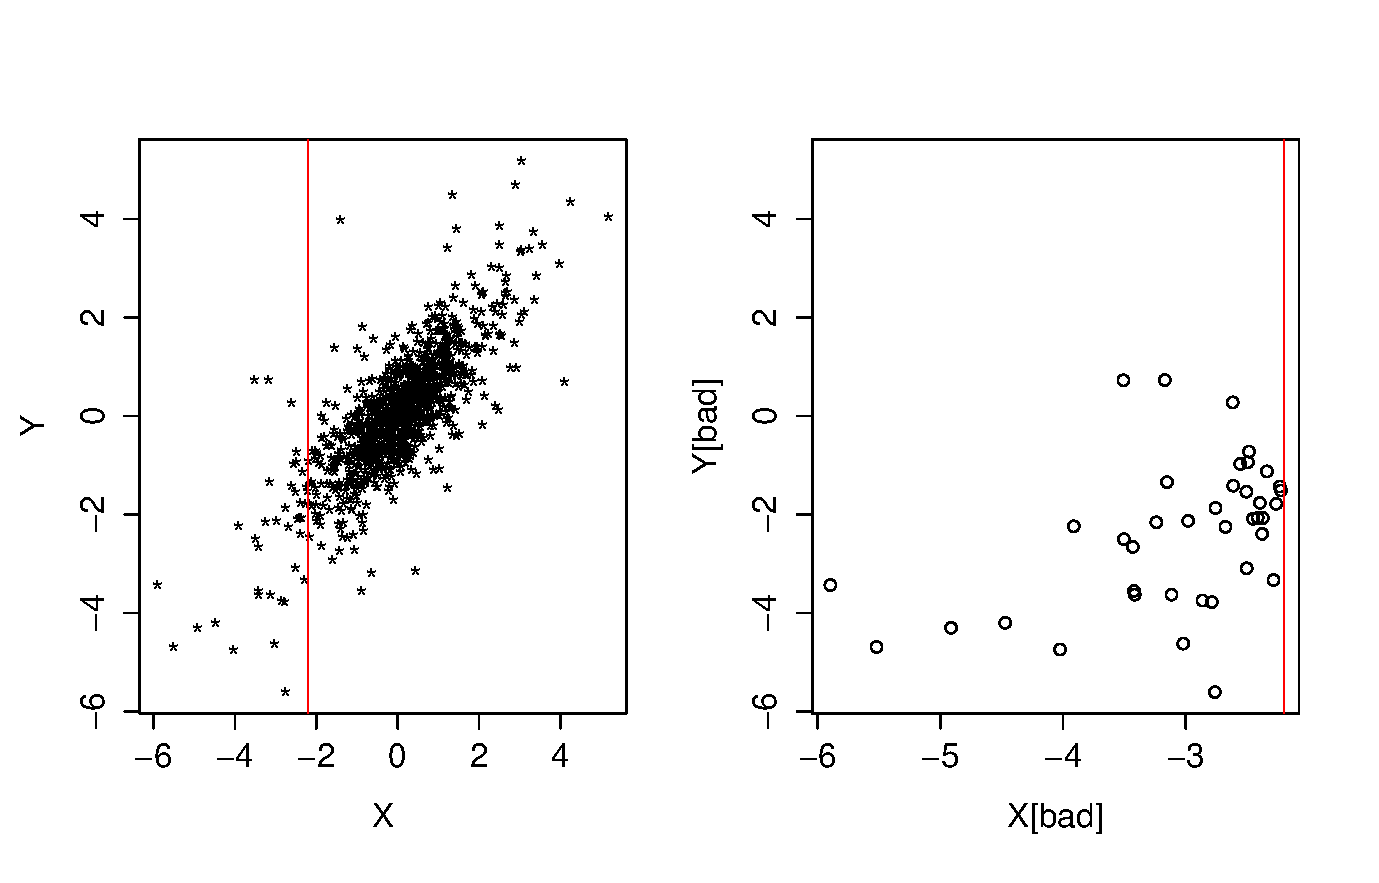
\includegraphics[scale=.6]{NL1_Q9_scatterplot.eps} 

We can see a tail dependence for the multiStudent distribution in the plot on the right hand side. The tail correlation of $0.44$ is lower than $0.8$, but is is a lot larger than $0$. This means that there is a tail dependence.

\subsection*{Q10}

Let $\vec{Z}$ be a correlated multinormal random vector with mean $\vec{\mu}$ and covariance matrix $\Sigma$. We denote $\rho$ as the correlation matrix and we use shorthand notation $\rho(Z_i,Z_j) = \rho_{i,j}$ and $\Cov(Z_i,Z_j) = \Sigma_{i,j}$.

By definition, $\rho(Z_i,Z_j) = \frac{\Cov(Z_i,Z_j)}{\sqrt{\Var[Z_i]\Var[Z_j]}}$. Using the shorthand, we derive $\Sigma$ to be.

\begin{align}
\Sigma_{i,j} & = \rho_{i,j} \sqrt{\Var[\vec{Z}_i]\Var[\vec{Z}]_j} \\
             & = \rho_{i,j} \sqrt{(\Var[\vec{Z}]\Var[\vec{Z}]^{T})_{i,j}} \\
\Sigma       & = \rho \sqrt{\Var[\vec{Z}]\Var[\vec{Z}]^{T}} \\
             & = \rho \sqrt{\Var[\vec{Z}] \otimes \Var[\vec{Z}]}
\end{align}

In the first step, we rewrite from index notation to vector notation as can be seen on the wikipedia page of the \href{https://en.wikipedia.org/wiki/Outer_product}{outer product}. We then drop the indexes and use that the outer product can be written as a matrix multiplication of a vector and its own transpose.

We execute the following code:

\begin{verbatim}
> library(MASS)
> mu <- c(1,3,5); sig2 <- c(1,2,5)
> Corrmat <- rbind(c(1., .3, .3),
+                  c(.3, 1., .4),
+                  c(.3, .4, 1.))
> Varmat <- Corrmat * sqrt(sig2 %*% t(sig2))
> Z <- mvrnorm(100, mu, Varmat)
> options(digits=7)
> colMeans(Z); diag(cov(Z)); cor(Z)
[1] 0.9497085 2.8927698 4.7217666
[1] 0.9276677 2.1010010 5.4895002
[,1]      [,2]      [,3]
[1,] 1.0000000 0.1696436 0.1025938
[2,] 0.1696436 1.0000000 0.4265725
[3,] 0.1025938 0.4265725 1.0000000
\end{verbatim}

\verb|colMeans(Z)| estimates the mean of each column. Therefore \verb|colMeans| should be close to the mean vector $\vec{\mu}$.
\verb|diag(cov(Z))| gives the diagonal elements of the covariance matrix. The diagonal elements of the covariance matrix contains the estimated variance of each element of $Z$. This should be close to $\Var[\vec{Z}]$ (or \verb|sig2|).
\verb|cor(Z)| contains the estimated correlation between the three elements of Z.

\subsection*{Q11}

We execute the following code in \verb|R|:

\begin{verbatim}
> no_sims = 1e6
> VaR <- rep(0,10)
> for (i in (1:10)){
+   Z <- mvrnorm(no_sims, mu, Varmat)
+   VaR[i] <- quantile(rowSums(Z),0.9999)
+ }
> VaR
[1] 22.34890 22.27627 22.24395 22.40076 22.29522 22.23880 22.33798 22.17733 22.32926 22.31303
> c(mean(VaR),sd(VaR))
[1] 22.29615014  0.06445194
\end{verbatim}

We are asked to determine the $F^{-1}_{Z}(0.9999)$, where $Z = Z_1 + Z_2 + Z_3$, with $Z_i$ as defined in question 10. Because $Z_i$ are random normally distributed, so is the sum $Z$. The mean of $Z$ is given by the following equation.

\begin{equation}
\E[Z] = \E[Z_1] + \E[Z_2] + \E[Z_3] = 1 + 3 + 5 = 9
\end{equation}

The variance is given by the following formula:

\begin{equation}
\Var[Z] = \Var[Z_1] + \Var[Z_2] + \Var[Z_2] + 2 (\Cov(Z_1,Z_2) + \Cov(Z_1,Z_3) + \Cov(Z_2,Z_3))
\end{equation}

The right hand side of this equation is equal to the sum of the elements of covariance matrix from the previous question. The theoretical value is then computed by executing the following code in R.

\begin{verbatim}
> Var_t <- qnorm(0.9999, sum(mu), sqrt(sum(Varmat)))
> Var_t
[1] 22.26391
\end{verbatim}

The estimated value of $22.296$ is close to the theoretical value of $22.264$.

\subsection*{Q12}

We generate $10^6$ independent drawings from a trinormal random vector $(X,Y,Z) \sim N(\vec{\mu} = \vec{0}; \Sigma)$, with the covariance matrix $\Sigma$ having ones on the diagonal and $\rho = 1/6$ outside the diagonal. Translated to \verb|R| this gives.

\begin{verbatim}
> n <- 1e6
> mu <- c(0,0,0)
> sigma <- rbind(c(1,1/6,1/6),
+                c(1/6,1,1/6),
+                c(1/6,1/6,1))
> Z <- mvrnorm(n, mu,sigma)
\end{verbatim}

\subsection*{Q13}

We construct $V_i = X_i + Y_i + Z_i$ by executing the following code in \verb|R|.

\begin{verbatim}
> V <- rowSums(Z)
\end{verbatim}

\subsection*{Q14}

We use the \verb|quantile| function to estimate the $97.5\%$ quantile $d = F^{-1}_{V}(0.975)$ by executing the following code in \verb|R|.

\begin{verbatim}
> d <- quantile(V,0.975)
> d
97.5% 
3.918903 
\end{verbatim}

The estimate for the $97,5\%$ quantile of \verb|V| is $3.92$.

\subsection*{Q15}

We execute the following code in \verb|R|, where we use the definition of the stoploss premium to estimate it for $V$ at level $97.5\%$.

\begin{verbatim}
> stoploss_premium <- mean(pmax(V-d,0)) 
> stoploss_premium
[1] 0.01884366
\end{verbatim}

The estimated stoploss premium is $0.0188$.

\subsection*{Q16}

By definition, the random variables $X_i$, $Y_i$ and $Z_i$ are normally distributed. The sum of normally distributed variables is also normally ditributed, therefore $V_i$ is also normally distributed. The mean and variance of $V_i$ can be obtained in the same manner as in question 11.

We run the following code in \verb|R| to obtain the mean and standard devation of $V_i$.

\begin{verbatim}
> mean <- sum(mu); sd <- sqrt(sum(sigma))
> c(mean, sd)
[1] 0 2
\end{verbatim}

\subsection*{Q17}

First, we calculate the theoretical value of $d$, after which we use formula $(3.104)$ from MART.

\begin{verbatim}
> d_new <- qnorm(0.975, mean, sd)
> stoploss_premium_mart <- sd * dnorm((d_new - mean)/sd) - (d_new - mean)*(1 - pnorm((d_new - mean)/sd))
> stoploss_premium_mart
[1] 0.01889194
\end{verbatim}

The theoretical stoploss premium of $0.01889$ is really close to its estimated value of $0.01884$.

\subsection*{Q18}

We use a sample size of $10^6$ toestimate the $ES$ of $V'$, where $V'$ is a sum of multi-student t random variables. The multi-normal random variables used to generate the student t variables have equal $\vec{\mu}$ and $\Sigma$ as in question $12$. The $\chi^2_k$ distribution used to transform the sum of normal variables into a student t variable has $5$ degrees of freedom. We then repeat the methods from questions $12$ to $15$.

\begin{verbatim}
> n <- 1e6
> k <- 5
> mu <- c(0,0,0)
> sigma <- rbind(c(1,1/6,1/6),
+                c(1/6,1,1/6),
+                c(1/6,1/6,1))
> Z <- mvrnorm(n, mu,sigma)
> chi5 <- sqrt(rchisq(n, df=5)/5)
> Z_prime <- Z/chi5
> V_prime <- rowSums(Z_prime)
> d <- quantile(V_prime,0.975)
> d
97.5% 
5.137715 
> stoploss_premium <- mean(pmax(V_prime-d,0)) 
> stoploss_premium
[1] 0.04811667
\end{verbatim}

We estimate the expected shortfall $ES = 0.0481$.

\subsection*{Q19}

A univariate Student(k) distribution is found by dividing $T \sim N(0,1)$ by a r.v. $\sqrt{U/k}$, with $U \sim \chi^2_k$, independent of $T$. We define $V = X + Y + Z$. $V$ is standard normally distributed with mean $\mu = 0$ and standard deviation $\sigma = 2$. The transform to a student distribution requires $\sigma = 1$, so we need to scale $V$ by sigma. We can then conclude that  $V/(\sigma \sqrt{(U/k)})$ has a student t distribution with k degrees of freedom. We define $V' = V/\sqrt{(U/k)}$, with cumulative distribution function $F_{V'}(x)$. It then follows that

\begin{equation}
F_{V'}(x) = \Pr[V' \le x] = \Pr[V/\sqrt{(U/k)} \le x] = \Pr[V/(\sigma \sqrt{(U/k)}) \le x/\sigma] = F_{st}(x/\sigma;k) 
\end{equation}

, where $F_{st}(x/\sigma;k)$ is the cumulative distribution function of the student distribution. We can now calculate the $97.5\%$ quantile $d$ by the following derivation.

\begin{equation}
F_{st}(d/\sigma;k) = 0.975 \implies d = \sigma F^{-1}_{st}(0.975;k) 
\end{equation}

Using formula (1.33) from MART, we can then determine the equation for the expected shortfall ES.

\begin{equation}
ES = \int_{d}^{\infty}[1-F_{st}(x/\sigma;k)]  dx
\end{equation}

We use the following functions in the next bit of \verb|R| code. \verb|qt()| gives the quantiles of the student t distribution, \verb|pt| is the distribution function of the student t distribution. 

\begin{verbatim}
> sd <- sqrt(sum(sigma))
> d_new <- sd * qt(0.975,5) 
> f <- function(x) {1 - pt(x/sd,5)}
> ES <- integrate(f, d_new, Inf)
> ES$value
[1] 0.04754977
\end{verbatim}

The theoretical value of $0.0475$ is very close to the estimated value of $0.0481$.